\documentclass[addpoints,12pt]{exam}

\usepackage{amsmath, amsthm, amssymb, amsfonts}
\usepackage{thmtools}
\usepackage{graphicx}
\usepackage[hidelinks]{hyperref}
\usepackage[utf8]{inputenc}
\usepackage[english]{babel}
\usepackage{framed}
\usepackage[dvipsnames]{xcolor}
\usepackage{tcolorbox}
\usepackage{tabto}
\usepackage{titling}
\usepackage{tikz}

\usepackage{changepage} % for the adjustwidth environment


\colorlet{LightGray}{White!90!Periwinkle}
\colorlet{LightOrange}{Orange!15}
\colorlet{LightGreen}{Green!15}

\newcommand{\HRule}[1]{\rule{\linewidth}{#1}}

\declaretheoremstyle[name=Theorem,]{thmsty}
\declaretheorem[style=thmsty,numberwithin=section]{theorem}
\tcolorboxenvironment{theorem}{colback=LightGray}

\declaretheoremstyle[name=Proposition,]{prosty}
\declaretheorem[style=prosty,numberlike=theorem]{proposition}
\tcolorboxenvironment{proposition}{colback=LightOrange}

\declaretheoremstyle[name=Principle,]{prcpsty}
\declaretheorem[style=prcpsty,numberlike=theorem]{principle}
\tcolorboxenvironment{principle}{colback=LightGreen}

%% This latex package provides all the utilities for
%% 15150 assignments development.
%% This package is intended to be included in writeup.tex at
%% problem level.
%% For a full list of custom commands, check 15150toolbox.md
%%
%% @author: Jolin Zhou
%% @email: jiulingz@andrew.cmu.edu

\NeedsTeXFormat{LaTeX2e}
\ProvidesPackage{toolbox-reduced}[2020/05/15 Latex toolbox for M20 Lecture Notes]

%%%%%%%%%%%%%%%%%%%%%
%% Robust Commands %%
%%%%%%%%%%%%%%%%%%%%%
% used throughout this package
\RequirePackage{etoolbox}
\RequirePackage{xparse}

% hyperlink/reference
\RequirePackage{xcolor}

% graphics
\RequirePackage{graphicx}

% emphasize
\usepackage{bm}
\DeclareTextFontCommand{\emph}{\bfseries\em}

%%%%%%%%%%%%%%%%%%%%%%%%%%%%%%%
%% Task related environments %%
%%%%%%%%%%%%%%%%%%%%%%%%%%%%%%%
% environment colors
\RequirePackage{xcolor}
\definecolor{task_color}      {RGB}{ 64, 100, 255}
\definecolor{solution_color}  {RGB}{  0,   0, 128}
\definecolor{constraint_color}{RGB}{175,   0,   0}

% task environment
\RequirePackage{framed}
\providerobustcmd{\attribute}[1]{}
\newcounter{taskcounter}
\NewDocumentEnvironment{task}{m}
{
  \stepcounter{taskcounter}
  \textbf{Task \arabic{taskcounter}.}\attribute{#1}
  \phantomsection
  \addcontentsline{toc}{subsubsection}{\textcolor{task_color}{\textbf{Task \arabic{taskcounter}.}\texorpdfstring{\attribute{#1}}{}}}
  \par
}
{
  \ifdef{\loadsolution}
    {{
      \color{solution_color}
      \begin{framed}
        \textbf{Solution \arabic{taskcounter}.}\par
        \loadsolution{#1}
      \end{framed}
    }}
    {}
  \vspace{1em}
}

% constraint environment
\newenvironment{constraint}{\color{constraint_color}\textbf{Constraint:}}{}

%%%%%%%%%%%%%%%%%%%%%%%%
%% Code Specification %%
%%%%%%%%%%%%%%%%%%%%%%%%
% spec
\RequirePackage{framed}
\usepackage{mdframed}
\newrobustcmd{\spec}[4]{
\begin{mdframed}
\code{#1 :}\code{#2}\par
\ifstrempty{#3}{}{\par REQUIRES: #3}
\ifstrempty{#4}{}{\par ENSURES: #4}
\end{mdframed}
}

%%%%%%%%%%%%%%%%%%%%%
%% Text Formatting %%
%%%%%%%%%%%%%%%%%%%%%
% symbols
\RequirePackage{amssymb, amsmath, amsthm, amsfonts}

\newrobustcmd{\stepsTo}{\Longrightarrow}
\newrobustcmd{\stepsToStar}{\Longrightarrow}
\newrobustcmd{\stepsToIn}[1]{\Longrightarrow^{#1}}

\newrobustcmd{\eeq}{\cong}

%%%%%%%%%%%%%%%%%%%%%%
%% Code Environment %%
%%%%%%%%%%%%%%%%%%%%%%
% code style
\RequirePackage{listings}
\RequirePackage{lstautogobble}
\RequirePackage{xcolor}

\newlength{\MaxSizeOfLineNumbers}%
\settowidth{\MaxSizeOfLineNumbers}{99}% Adjust to maximum number of lines
\addtolength{\MaxSizeOfLineNumbers}{.5ex}%

\newcommand{\darkBg}{8b98ad}
\definecolor{background_color}{RGB}{225, 225, 225}
\definecolor{string_color}    {RGB}{180, 156,   0}
\definecolor{keyword_color}   {RGB}{ 64, 100, 255}
\definecolor{comment_color}   {RGB}{  140, 140, 140}
\definecolor{number_color}    {RGB}{ 84,  84,  84}
\lstdefinestyle{15150code}{
    basicstyle=\ttfamily,
    numberstyle=\tiny\ttfamily\color{number_color},
    stringstyle=\color{string_color},
    keywordstyle=\color{blue!90!black},
    commentstyle=\color{comment_color},
    numbers=left,
    rulesepcolor=\color{black!20!white},
    linewidth=\textwidth,
    columns=fixed,
    tabsize=2,
    xleftmargin=\MaxSizeOfLineNumbers,
    breaklines=true,
    keepspaces=true,
    showstringspaces=false,
    captionpos=b,
    autogobble=true,
    mathescape=true,
    literate={~}{{$\thicksim$}}1
             {~=}{{$\eeq$}}1
}
\lstdefinelanguage{sml}{
    language=ML,
    morestring=[b]",
    morecomment=[s]{(*}{*)},
    morekeywords={
        bool, char, exn, int, real, string, unit, list, option,
        EQUAL, GREATER, LESS, NONE, SOME, nil,
        andalso, orelse, true, false, not,
        if, then, else, case, of, as,
        let, in, end, local, val, rec,
        datatype, type, exception, handle,
        fun, fn, op, raise, ref,
        structure, struct, signature, sig, functor,
        include, open, use, infix, infixr, o, print
    }
}

\usepackage[T1]{fontenc}

\makeatletter
\newenvironment{btHighlight}[1][]
{\begingroup\tikzset{bt@Highlight@par/.style={#1}}\begin{lrbox}{\@tempboxa}}
{\end{lrbox}\bt@HL@box[bt@Highlight@par]{\@tempboxa}\endgroup}

\newcommand\btHL[1][]{%
  \begin{btHighlight}[#1]\bgroup\aftergroup\bt@HL@endenv%
}
\def\bt@HL@endenv{%
  \end{btHighlight}%
  \egroup
}
\newcommand{\bt@HL@box}[2][]{%
  \tikz[#1]{%
    \pgfpathrectangle{\pgfpoint{1pt}{0pt}}{\pgfpoint{\wd #2}{\ht #2}}%
    \pgfusepath{use as bounding box}%
    \node[anchor=base west, fill=yellow!45,outer sep=0pt,inner xsep=1pt, inner ysep=0pt, rounded corners=3pt, minimum height=\ht\strutbox+1pt,#1]{\raisebox{1pt}{\strut}\strut\usebox{#2}};
  }%
}

\newenvironment{atHighlight}[1][]
{\begingroup\tikzset{at@Highlight@par/.style={#1}}\begin{lrbox}{\@tempboxa}}
{\end{lrbox}\at@HL@box[at@Highlight@par]{\@tempboxa}\endgroup}

\newcommand\atHL[1][]{%
  \begin{atHighlight}[#1]\bgroup\aftergroup\at@HL@endenv%
}
\def\at@HL@endenv{%
  \end{atHighlight}%
  \egroup
}
\newcommand{\at@HL@box}[2][]{%
  \tikz[#1]{%
    \pgfpathrectangle{\pgfpoint{1pt}{0pt}}{\pgfpoint{\wd #2}{\ht #2}}%
    \pgfusepath{use as bounding box}%
    \node[anchor=base west, fill=red!45,outer sep=0pt,inner xsep=1pt, inner ysep=0pt, rounded corners=3pt, minimum height=\ht\strutbox+1pt,#1]{\raisebox{1pt}{\strut}\strut\usebox{#2}};
  }%
}
\makeatother

% code inline
\newrobustcmd{\code}[2][]{{\sloppy
\ifmmode
    \text{\lstinline[language=sml,style=15150code,#1]`#2`}
\else
    {\lstinline[language=sml,style=15150code,#1]`#2`}%
\fi}}

% code block
\lstnewenvironment{codeblock}[1][]{\lstset{
  language=sml,
  style=15150code,numbers=none,#1,moredelim=**[is][\btHL]{`}{`},moredelim=**[is][\atHL]{&}{&}}}{}

% ------------------------------------------------------------------------------

\usepackage{fancyhdr}
\begin{document}

% Set the page style to "fancy"...
\pagestyle{fancy}
%... then configure it.
\fancyhead{} % clear all header fields
\fancyhead[R]{15-150: Principles of Functional Programming}
\fancyhead[L]{Midterm 2 (2)}
\fancyfoot[C]{\thepage} % clear all footer fields

% ------------------------------------------------------------------------------
% Cover Page and ToC
% ------------------------------------------------------------------------------

\setlength{\droptitle}{-8em}   % This is your set screw

\title{ \normalsize \textsc{}
		\HRule{1.5pt} \\
		\large \textbf{
      \uppercase{Midterm 2 (2)} \\
      15-150 Principles of Functional Programming M23} \\
    \HRule{1.5pt}
    \date{}
}

\maketitle

\vspace{-3cm}

\hspace{-1cm} Name \rule{5cm}{0.4pt} \, Andrew ID \rule{3cm}{0.4pt} \, House \rule{3.5cm}{0.4pt}

\vspace{5pt}

\begin{itemize}
  \item Write your name, Andrew ID, and House name on this page.
  \item This is an 80 minute examination of 6 parts.
  \item Answers should be short and to the point. Obey question constraints, wherever
  they appear, and write syntactically legal SML programs!
  \item At any point on this examination, you are allowed to use the \code{map},
  \code{filter}, \code{foldl}, \code{foldr}, \code{length}, and \code{|>} functions,
  as seen in lecture. You may also use the identity function as \code{id}.
\end{itemize}
\vspace{\fill}

{\small
\vqword{}
\vpword{Max}
\begin{center}
\gradetable[v][questions]
\end{center}
}

\vspace{\fill}

\begin{center}
  Feel free to use this space to draw a joke or meme about functional programming: \\

  \vspace{10pt}

  \fbox{\rule{6in}{0pt}\rule[-0.5ex]{0pt}{2.5in}}
\end{center}


\newpage

% ------------------------------------------------------------------------------

\section*{Questions}

\begin{questions}

\titledquestion{Types and Values}
\textbf{Types and Values}

For each of the expressions below, write its \textbf{most general type} and value.

\textbf{If the expression is not well-typed then say so and explain your answer briefly.}

\textbf{If the expression does not evaluate to a value then say so and explain your answer briefly.}

\textbf{For brevity, if the expression is already a value, you may write out "same" for its value}.

\begin{parts}

  \part[2]\hfill

  \begin{codeblock}
    fn x => fn y => fn z =>
      if x then
        z (y, y)
      else
        z x
  \end{codeblock}

  \textbf{Type:} \begin{solutionorlines}[2em] NWT \end{solutionorlines}

  \textbf{Value:} \begin{solutionorlines}[2em] no value, not well typed \end{solutionorlines}

  \vspace{10pt}

  \part[2]\hfill

  \begin{codeblock}
    fn x => (x, x)
  \end{codeblock}

  \textbf{Type:} \begin{solutionorlines}[2em] \code{'a -> 'a * 'a} \end{solutionorlines}

  \textbf{Value:} \begin{solutionorlines}[2em] \code{fn x => (x, x)} \end{solutionorlines}

  \vspace{10pt}

  \newpage

  \part[2]\hfill

  \begin{codeblock}
    Node (
      Empty,
      Node (
        Empty,
        [],
        Empty
      ),
      Empty
    )
  \end{codeblock}

  \textbf{Type:} \begin{solutionorlines}[2em] \code{'a list tree tree} \end{solutionorlines}

  \textbf{Value:} \begin{solutionorlines}[2em] \code{Node (Empty, Node (Empty, [], Empty), Empty)} \end{solutionorlines}

  \vspace{10pt}

  \part[2]\hfill

  \begin{codeblock}
    (fn x => fn y => fn z => (x ^ y, z y)) "here" "kitty"
  \end{codeblock}

  \textbf{Type:} \begin{solutionorlines}[2em] \code{(string -> 'a) -> (string * 'a)} \end{solutionorlines}

  \textbf{Value:} \begin{solutionorlines}[2em] \code{fn z => ("here" ^ "kitty", z "kitty")} \end{solutionorlines}

\end{parts}

\newpage

\titledquestion{Evaluation and Equivalence}

\textbf{Evaluation and Equivalence}

For each of the questions below, please mark whether they are "true" or
"false". If your answer is false, please briefly justify why.

\begin{parts}
  \part[2]\hfill

  Given \code{g : (t1 -> t2) -> t3}, if \code{f : t1 -> t2} is total, then
  \code{g f} is valuable.

  \begin{solutionorlines}[4em] False. Consider \code{fn _ => 1 div 0}. \end{solutionorlines}

  \part[2]\hfill

  For any \code{f : t1 -> t2 -> t3}, \code{f} is total.

  \begin{solutionorlines}[4em] False, consider \code{fn _ => raise Div} \end{solutionorlines}

  \part[2]\hfill

  \code{foldr (fn (x, acc) => f x :: acc) [] L} $\eeq$ \code{map f L}, for an \\
  arbitrary \code{f : t1 -> t2} and \code{L : t1 list}.

  \begin{solutionorlines}[4em] False, in the presence of exceptions. \code{foldr}
  goes from the right, so this may cause exceptions to be raised in a different
  order. \end{solutionorlines}

  \part[5]\hfill

  Consider the following code:

  \begin{codeblock}
    exception Fact of int

    fun factCPS 0 k = k (raise Fact 1)
      | factCPS n k =
          factCPS (n - 1) (fn res =>
            res handle Fact res' => k (n * res')
          )

    fun fact n = factCPS n (fn x => x handle Fact res => res)
  \end{codeblock}

  True or false, this is a correct implementation of \code{fact}.

  \begin{solutionorlines}[4em] False, the exception \code{Fact} is never
  actually handled. \end{solutionorlines}

  \newpage

  \part[2]\hfill

  Consider the following expression:
  \begin{codeblock}
    plus 2 (mul 3 (plus 1 0))
  \end{codeblock}

  Suppose you are given \code{plusCPS}, and \code{mulCPS}
  that take in an additional continuation as an argument. True or false,
  this is the correct way to translate this code to CPS:

  \begin{codeblock}
    plusCPS 1 0  (fn res =>
    mulCPS 3 res (fn res2 =>
    plusCPS 2 res2  ))
  \end{codeblock}

  \begin{solutionorlines}[4em]
    False, \code{plusCPS} is not given a continuation.
  \end{solutionorlines}

\end{parts}

\newpage
\titledquestion{Cool Trees}

\textbf{Cool Trees}

Consider the following datatype for \textit{cool trees}.
\begin{codeblock}
  datatype 'a cool =
      Empty
    | Node of 'a cool * 'a * 'a cool
    | Leaf of 'a
\end{codeblock}

In this section, we are going to be solving the problem of
\textit{subtree equivalence}. This is the problem of, given
two trees, trying to find all subtrees of the second tree which
are equivalent to the first tree.

For instance, given the following two cool trees:

\begin{center}
  \begin{minipage}{0.3\textwidth}
    \begin{center}
      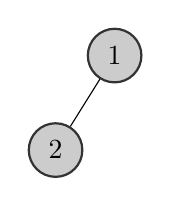
\begin{tikzpicture}
        [level distance=12mm,
        every node/.style={circle,inner sep=4pt, draw=black!80, thick},
        ]
        \node[fill=black!20!white] {1}
          child {node[fill=black!20!white] {2}}
          child[missing];
        \end{tikzpicture}
    \end{center}
  \end{minipage}
  \begin{minipage}{0.3\textwidth}
  \begin{center}
    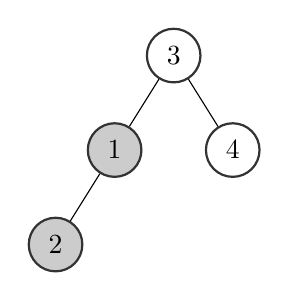
\begin{tikzpicture}
      [level distance=12mm,
      every node/.style={circle,inner sep=4pt, draw=black!80, thick},
      ]
      \node {3}
        child {node[fill=black!20!white] {1}
          child{node[fill=black!20!white]{2}}
          child[missing]
        }
        child {node {4}};
      \end{tikzpicture}
  \end{center}
  \end{minipage}
\end{center}
the grey nodes in both trees are equivalent trees.
The second tree has only a single subtree which is equivalent to the first tree.

\begin{parts}
  \part[5]\hfill

    Before we can solve the problem of subtree equivalence, we need to define what
    it means for two trees to be equivalent. With the
    \code{'a tree} type that we saw in lecture, this is an easy question to answer,
    because they are only equal when their tree values are literally equal, according
    to some equality function on elements.

    Cool trees are a little different because they allow a \code{Leaf} case.
    We'd like to say that this is a little redundant, because a \code{Leaf x}
    tree is pretty much the same thing as \code{Node (Empty, x, Empty)}. In
    this case, we say that these two trees are \textit{equivalent}.

    Implement the following function:

    \spec
      {coolEquiv}
      {('a * 'a -> bool) -> 'a cool -> 'a cool -> bool}
      {\code{eq} is total}
      {\code{coolEquiv eq T1 T2} $\eeq$ \code{true} iff \code{T1} and
      \code{T2} are equivalent cool trees, by the discussion above.}

    So, for instance:
    \begin{codeblock}
      val N = Node
      val E = Empty

      val true  = coolEquiv (op=) E E
      val false = coolEquiv (op=) E (N (E, 1, E))
      val true  = coolEquiv (op=) (Leaf 1) (N (E, 1, E))
      val false = coolEquiv (op=) (Leaf 2) (N (E, 1, E))
      val false = coolEquiv (op=) (N (E, 2, E)) (N (E, 1, E))
      val false =
        coolEquiv (fn _ => false) (N (E, (), E)) (N (E, (), E))
    \end{codeblock}

    Please fill in the missing cases in the below implementation of
    \code{coolEquiv}. This can be done in four cases.

    \begin{codeblock}
      fun coolEquiv eq Empty Empty = true
        (* FILL IN BELOW! *)
    \end{codeblock}
    \begin{solutionorbox}[25em]
      \begin{codeblock}
          | coolEquiv eq (Leaf x) (Leaf x') = eq x x'
          | coolEquiv eq (Node (Empty, x, Empty)) (Leaf x') = eq x x'
          | coolEquiv eq (Leaf x) (Node (Empty, x', Empty)) = eq x x'
          | coolEquiv eq (Node (L, x, R)) (Node (L', x', R')) =
              coolEquiv L L' andalso eq x x' andalso coolEquiv R R'
      \end{codeblock}
    \end{solutionorbox}
    \begin{codeblock}
      (* FILL IN ABOVE! *)
        | coolEquiv eq _ _ = false
    \end{codeblock}

  \newpage
  \part[8]\hfill

    Now, let's complete the problem. Suppose you are given the function \\
    \code{subtrees : 'a cool -> 'a cool list}, which simply computes all of the subtrees of a given cool
    tree. For instance, it may be implemented like so:

    \begin{codeblock}
      fun subtrees Empty = [Empty]
        | subtrees (Leaf x) = [(Leaf x)]
        | subtrees (Node (L, x, R)) =
            subtree L @ ((Node (L, x, R)) :: subtrees R)
    \end{codeblock}

    Using \code{subtrees} and
    \code{coolEquiv}, implement a function with the following specification:

    \spec
      {matchSubtrees}
      {('a * 'a -> bool) -> 'a cool -> 'a cool -> 'a cool list}
      {\code{eq} is total}
      {\code{matchSubtrees eq T1 T2} evaluates to all of the subtrees
      of \code{T2} that are equivalent to \code{T1}}

    \begin{constraint}
      To get full points for this problem, you cannot use any lambda expressions.
    \end{constraint}

    \begin{solutionorbox}[25em]
      \begin{codeblock}
        fun matchSubtrees eq T1 T2 =
          subtrees T2
          |> List.filter (coolTreeEq eq T1)
      \end{codeblock}
    \end{solutionorbox}

  Congratulations. You basically just implemented what I do for Semgrep
  as a \\ software engineer.
\end{parts}

\newpage
\titledquestion{Binary Search Trees, Again}

\textbf{Binary Search Trees, Again}

Recall the type of integer \code{tree}s, from lecture:
\begin{codeblock}
  datatype tree = Empty | Node of tree * int * tree
\end{codeblock}

A \textit{binary search tree} is a value of type \code{tree}, that satisfies the
following definition:

\textbf{Definition.} A value \code{v : t} is called a \textit{binary search tree} if:
\begin{enumerate}
  \item It is \code{Empty}.
  \item It is \code{Node (L, x, R)}, where both \code{L} and \code{R} are binary
  search trees, and \code{x} is greater than or equal to every
  element in \code{L}, and less than or equal to every element in \code{R}.
\end{enumerate}

\begin{parts}
  \part[12]\hfill

  First, we will define a helper function:

  Implement a function \code{isBST'} which adheres to the following specification:

  \spec
    {isBST'}
    {(int -> bool) -> tree -> (bool -> 'a) -> 'a}
    {\code{p} is total}
    {\code{isBST' p T k} evaluates to \code{k true} if \code{T} is a binary
    search tree, and every element in \code{T} satisfies \code{p}. Otherwise,
    it evaluates to \code{k false}.}

  \begin{constraint}
    You must write this function in CPS, and with no helper functions.
  \end{constraint}

  \begin{solutionorbox}[25em]
    \begin{codeblock}
      fun isBST' p Empty k = k true
        | isBST' p (Node (L, x, R)) k =
            isBST' (fn y => y <= x) L (fn is_bst_l =>
            isBST' (fn y => x <= y) R (fn is_bst_r =>
            k (is_bst_l andalso is_bst_r andalso p x)))
    \end{codeblock}
  \end{solutionorbox}

  \newpage

  \part[2]\hfill

  Implement a function \code{isBST''}, using \code{isBST'}, with the following
  specification:

  \spec
    {isBST''}
    {tree -> (bool -> 'a) -> 'a}
    {\code{true}}
    {\code{isBST'' T k} evaluates to \code{k true} if \code{T} is a binary
    search tree. Otherwise, it evaluates to \code{k false}.}

  \begin{constraint}
    For full points, do not use a \code{fun} declaration.
    You may use precisely one lambda expression.
  \end{constraint}

  \begin{solutionorbox}[20em]
    \begin{codeblock}
      val isBST'' = isBST' (fn x => true)
    \end{codeblock}
  \end{solutionorbox}
\end{parts}

\newpage
\titledquestion{Code Cleanup}

\textbf{Code Cleanup}

Brandon is writing code to deal with his 150 grades database, but
accidentally wrote it very redundantly!\footnotemark His code is:

\begin{codeblock}
  type grades = (string * int) list

  (* DISCLAIMER: NOT NECESSARILY INDICATIVE OF HOW YOU WILL
     ACTUALLY BE GRADED IN THIS COURSE
   *)

  fun getAStudents ([] : grades) = ([], [])
    | getAStudents ((student, grade)::xs) =
        let
          val (agrades, nagrades) = getAStudents xs
        in
          if grade >= 90 then
            (student :: agrades, nagrades)
          else
            (agrades, student :: nagrades)
        end

  fun getBStudents ([] : grades) = ([], [])
    | getBStudents ((student, grade)::xs) =
        let
          val (bgrades, nbgrades) = getBStudents xs
        in
          if grade >= 80 then
            (student :: bgrades, nbgrades)
          else
            (bgrades, student :: nbgrades)
        end

  fun getCStudents ([] : grades) = ([], [])
    | getCStudents ((student, grade)::xs) =
        let
          val (cgrades, ncgrades) = getCStudents xs
        in
          if grade >= 70 then
            (student :: cgrades, ncgrades)
          else
            (cgrades, student :: ncgrades)
        end
\end{codeblock}

\footnotetext[1]{Joke's on you, this is an exam problem, I would never do this. I am perfect.}

\newpage

\begin{parts}
  \part[2]\hfill

  Identify the one significant difference between \code{getAStudents},
  \code{getBStudents}, and \code{getCStudents}. Do not count names of variables.

  \begin{solutionorbox}[10em]
    They use different hard-coded thresholds for where to separate the students.
  \end{solutionorbox}

  \part[8]\hfill

  Come up with a function \code{f} such that \code{f} encapsulates
  the same logic as all of the functions \code{getAStudents},
  \code{getBStudents}, and \code{getCStudents}, but "factors out"
  your answer from the previous part. Your answer should have a
  different type.

  \begin{constraint}
    Your function cannot be recursive.
  \end{constraint}

  \begin{solutionorbox}[30em]
    \begin{codeblock}
      fun partitionGrades threshold L =
        foldr (fn ((student, grade), (above, below)) =>
          if grade >= threshold then
            (student :: above, below)
          else
            (above, student :: below)
        ) ([], [])
    \end{codeblock}
  \end{solutionorbox}

  \part[2]\hfill

  Define the \code{getAStudents} function in terms of your function \code{f}.

  \begin{solutionorbox}[20em]
    \begin{codeblock}
      val getAStudents = partitionGrades 90
    \end{codeblock}
  \end{solutionorbox}
\end{parts}

\newpage
\titledquestion{Bounded Regular Expressions}

\textbf{Bounded Regular Expressions}

Consider the following extension of the \code{regexp} datatype, as
shown in lecture:

\begin{codeblock}
  datatype regexp =
      Zero
    | One
    | Char of char
    | Times of regexp * regexp
    | Plus of regexp * regexp
    | Star of regexp
    | Bounded of int * regexp
\end{codeblock}

We have introduced a new \code{Bounded} operator which has the following
mathematical description:

$$s \in L(\code{Bounded(n, r)}) \iff s \in L(r) \, \land \, s \text{ is at most \code{n} characters long}$$

\begin{parts}
  \part[10]\hfill

  Implement only the \code{Bounded} case for the \code{match} function, on
  the next page. The entire \code{match} function is duplicated there for your
  convenience.

  \vspace{160pt}

  THIS SPACE INTENTIONALLY LEFT BLANK

  \newpage

  \begin{EnvUplevel}
  \setlength{\leftmargin}{0pt}
  \begin{codeblock}
  fun match (r : regexp)
            (cs : char list)
            (k : char list -> bool) : bool =
    case r of
      Zero => false
    | One => k cs
    | Char c => (case cs of
        [] => false
      | c' :: cs' => c = c' andalso k cs')
    | Plus (r1,r2) => match r1 cs k orelse match r2 cs k
    | Times (r1, r2) => match r1 cs (fn cs' => match r2 cs' k)
    | Star r =>
        k cs orelse
        match r cs (fn cs' =>
          cs' <> cs andalso match (Star r) cs' k
        )
    | Bounded (n, r) =>
        (* FILL IN HERE! *)
  \end{codeblock}
  \end{EnvUplevel}
  \begin{solutionorbox}[25em]
    \begin{codeblock}
        match r cs (fn cs' =>
          if length cs - length cs' <= n then
            k cs'
          else
            false
        )
    \end{codeblock}
  \end{solutionorbox}
\end{parts}

\end{questions}




\begin{comment}
\section{Types and Values}

Please write the type and value of each given expression,
if applicable. If the expression does not have a type, please give a brief
justification as to why.
If the expression is not valuable, please give a brief justification as to
why.

\vspace{5pt}

\task{1}
\begin{codeblock}
  fn x => x + 2
\end{codeblock}

\vspace{10pt}

Type \rule{12cm}{0.4pt}

\vspace{10pt}

Value \rule{12cm}{0.4pt}

\vspace{15pt}

\task{2}
\begin{codeblock}
  fn x => x + 2
\end{codeblock}

\vspace{10pt}

Type \rule{12cm}{0.4pt}

\vspace{10pt}

Value \rule{12cm}{0.4pt}

\vspace{15pt}

\task{3}
\begin{codeblock}
  fn x => x + 2
\end{codeblock}

\vspace{10pt}

Type \rule{12cm}{0.4pt}

\vspace{10pt}

Value \rule{12cm}{0.4pt}

\vspace{15pt}

\task{4}
\begin{codeblock}
  fn x => x + 2
\end{codeblock}

\vspace{10pt}

Type \rule{12cm}{0.4pt}

\vspace{10pt}

Value \rule{12cm}{0.4pt}

\vspace{15pt}

\task{5}
\begin{codeblock}
  fn x => x + 2
\end{codeblock}

\vspace{10pt}

Type \rule{12cm}{0.4pt}

\vspace{10pt}

Value \rule{12cm}{0.4pt}

\vspace{15pt}

\newpage

\begin{theorem}
    This is a theorem.
\end{theorem}

\begin{proposition}
    This is a proposition.
\end{proposition}

\begin{principle}
    This is a principle.
\end{principle}

% Maybe I need to add one more part: Examples.
% Set style and colour later.

\subsection{Pictures}
\end{comment}

% ------------------------------------------------------------------------------

\end{document}